
A interface gráfica consiste de um menu com diferentes opções de controle e visualização dos sinais do sistema e um conjunto de gráficos dinâmicos para visualizar os estados do sistema em tempo real. A figura \ref{fig3:image_14} mostra a interface do sistema. No entanto, além da parte visual existe a parte de aquisição e processamento de dados, em TI essa parte e chamada de Back-end, o projeto possui uma classe para realizar essa parte de aquisição e tratamento de dados, além de uma classe para detectar automaticamente o microcontrolador conectado a porta USB.

Para ser possível realizar os ensaios, modificação de parâmetros do sinal de referência e coletas de dados é preciso que o microcontrolador execute o firmware, subseção \ref{firmware}, desenvolvido especificamente para esse propósito, dessa forma, a interface gráfica, figura \ref{fig3:image_14}, conseguirá realizar o pre-processamentos dos dados e plotar os sinais nos gráficos e demais atualizações nos softwares.

\begin{figure}[!h]
	\centering
	\caption{Interface Gráfica.}
	\efbox{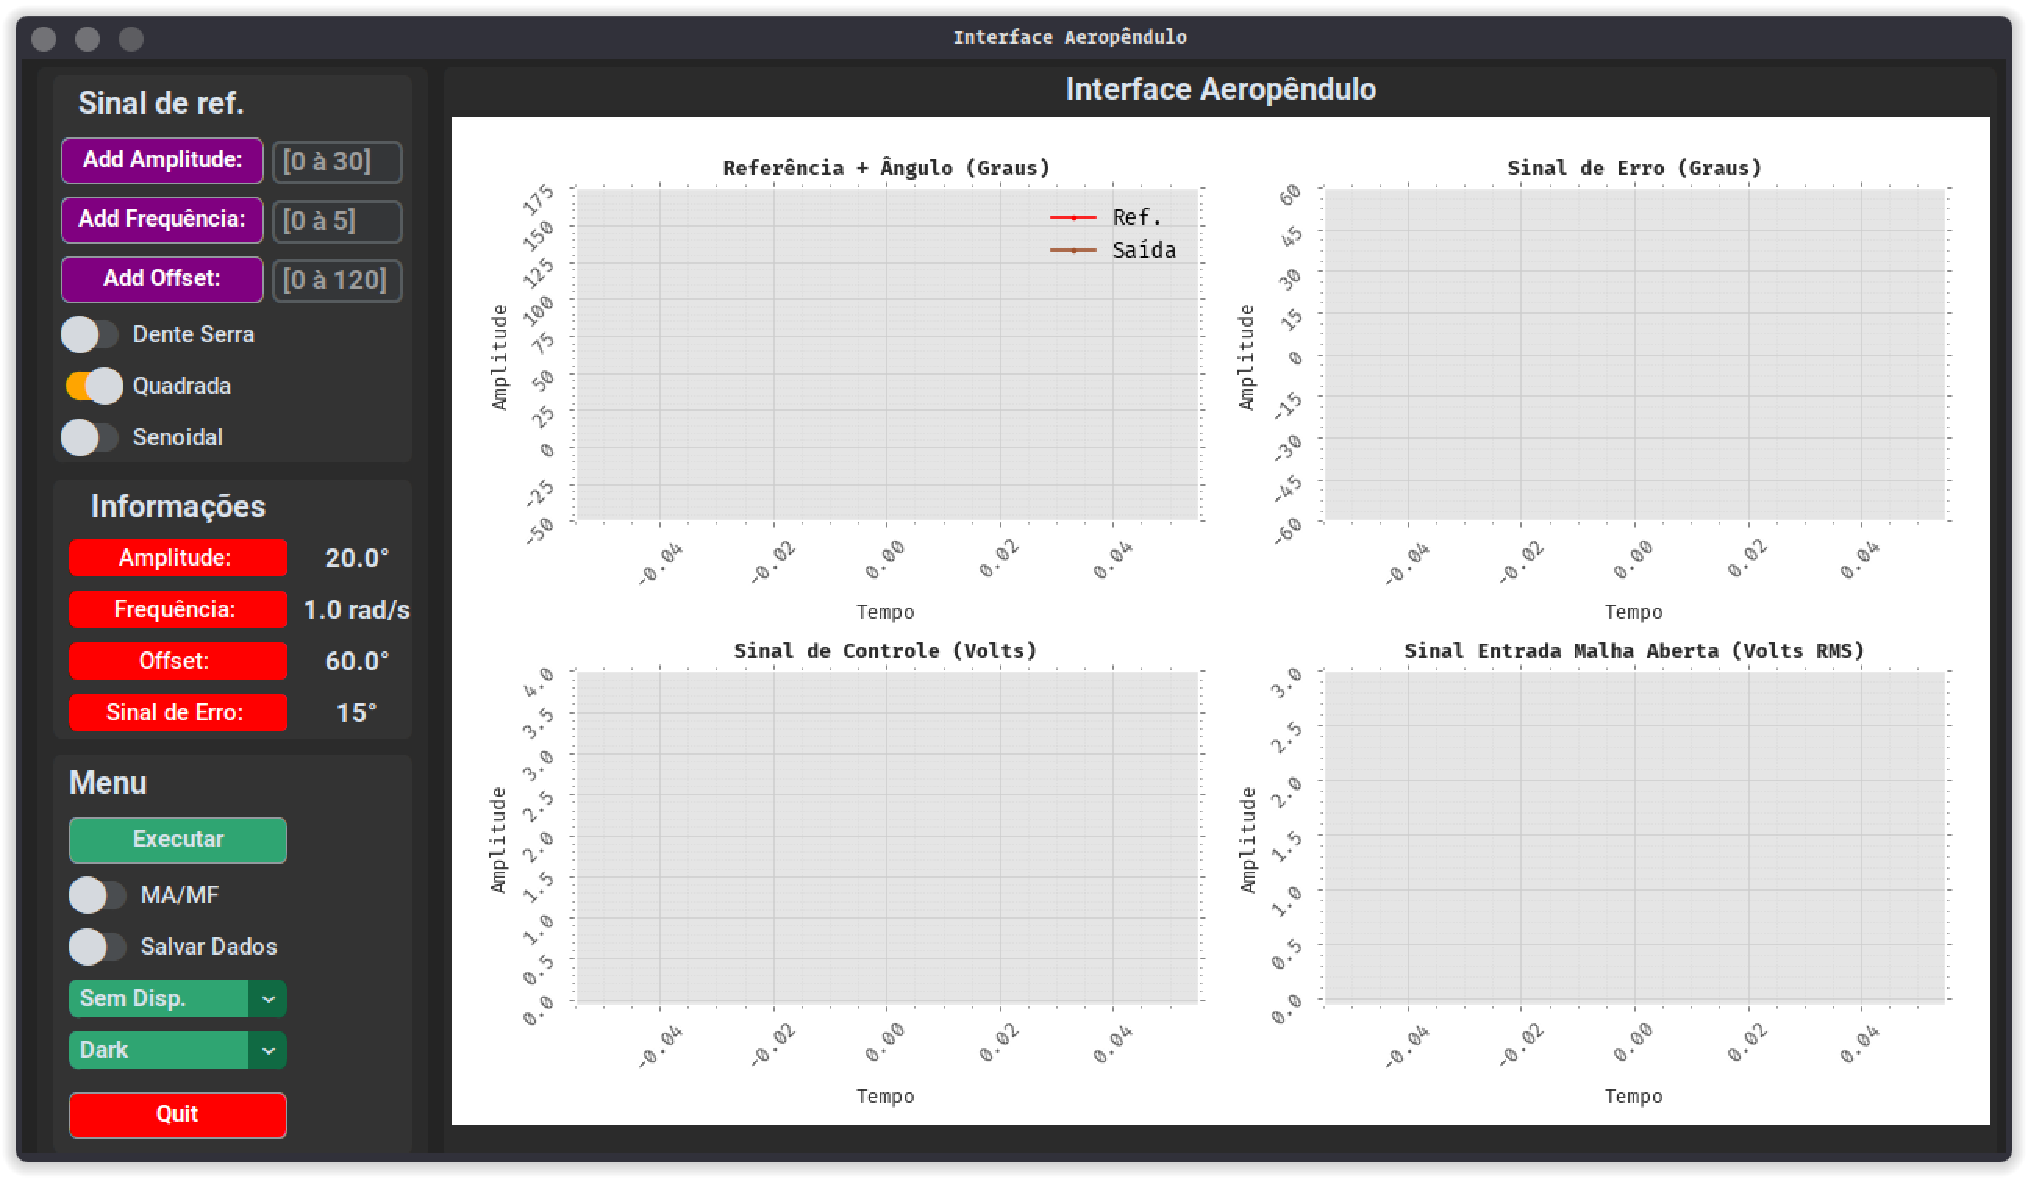
\includegraphics[width=0.9\textwidth]{Capitulos/3_hardware_softwares/3_figuras/interface.pdf}}
        \vspace{0.001cm}
	\caption*{Fonte: elaborado pelo autor (2023).}
	\label{fig3:image_14}
\end{figure}



O código a seguir realiza a importação de todos os módulos Python desenvolvidos tanto para a implementação da Interface Gráfica do Usuário quanto para o Gêmeo Digital. Com base nisso, foi elaborado um algoritmo que organiza adequadamente o funcionamento de ambos os softwares, viabilizando uma comunicação eficiente entre eles.

\vspace{0.5cm}

\begin{lstlisting}[language=python, numbers=left, label=py2, caption={Código que execulta a Interface Gráfica e o Gêmeo Digital.}]
import argparse
# Modulos da Interface Grafica de Usuario
from src_interface import InterfaceAeropendulo
from src_interface.graficos_sinais import GraficosSinais

# Modulos do Gemeo Digital
from simulador_aeropendulo.simulador import Simulador
from simulador_aeropendulo.graficos_aeropendulo import Graficos
from simulador_aeropendulo import AnimacaoAeropendulo

class RunInterface:
    def __init__(self) -> None:
        simular = self.get_args()
        self.runinterface(simular)

    def get_args(self) -> bool:
        parser = argparse.ArgumentParser()
        parser.add_argument(
            "-simular", "--Output",
            help="""Para habilitar o simulador, use a sintax:
                    python rungui.py -simular sim""")
        args = parser.parse_args()
        if args.Output == "sim":
            return True
        else:
            return False

    def runinterface(self, simular):
        if simular:
            simulador = Simulador(Graficos(), AnimacaoAeropendulo())
        else:
            simulador = None
        InterfaceAeropendulo(GraficosSinais,
                             simulador, baud_rate=115200,
                             amostras=80.0, tela_fixa=True)

if __name__ == "__main__":
    RunInterface()

\end{lstlisting}


Para roda a Interface Gráfica de Usuário juntamente com o Gêmeo Digital usa-se o seguinte comando no terminal estando dentro da pasta a partir do terminal:

\vspace{0.5cm}

\begin{lstlisting}[language=python]
python rungui.py -simular sim
\end{lstlisting}

Para roda apenas a Interface Gráfica de Usuário usa-se o seguinte comando no terminal:

\vspace{0.5cm}

\begin{lstlisting}[language=python]
python rungui.py
\end{lstlisting}



\subsubsection{Biblioteca CustomTkinter e Matplotlib}

Para o desenvolvimento da parte gráfica do software foi usado as bibliotecas CustomTkinter e Matplotlib, onde a biblioteca CustomTkinter implementa a estrutura de tela, botões, entradas de texto da aplicação e os módulos \textit{Matplotlib.pyplot} e \textit{Matplotlib.animation} possibilitam gerar gráficos em tempo real em conjunto com CustomTkinter.

Conforme \cite{customtkinter} explica no site oficial da biblioteca, "CustomTkinter é uma biblioteca de UI de desktop python baseada em Tkinter, que fornece widgets de aparência moderna e totalmente personalizáveis. Com CustomTkinter você terá uma aparência consistente em todas as plataformas de desktop (Windows, macOS, Linux)."

De acordo com \cite{matplotlib}, "Matplotlib é uma biblioteca abrangente para criar visualizações estáticas, animadas e interativas em Python. Matplotlib torna as coisas simples fáceis e as difíceis possíveis."

\subsubsection{Biblioteca PySerial, NumPy e Pandas}
Já para implementar o Back-end foram utilizadas as bibliotecas PySerial, NumPy e Pandas. Sendo que a biblioteca PySerial tem por finalidade realizar a comunicação entre o computador e o microcontrolador usando o protocolo seial via entrada USB, já o NumPy teve sua aplicação no processo de criação das matrizes contendo os dados lidos pela PySerial, por fim, para salvar os dados de ensaio foi usada a biblioteca Pandas, sendo salvos no formato CSV.

Conforme \cite{pyserial}, "A biblioteca PySerial possibilita a comunicação serial entre o computador e o microcontrolador usando conexão USB, Este módulo encapsula o acesso à porta serial. Ele fornece backends para Python rodando em Windows, OSX, Linux, BSD (possivelmente qualquer sistema compatível com POSIX) e IronPython. O módulo denominado “serial” seleciona automaticamente o backend apropriado."

% \citeonline[p.~11]{numpy_opl}   - Exemplo

De acordo com \cite{numpy_opl}, "O NumPy, uma biblioteca essencial para Python, oferece recursos robustos para realizar cálculos numéricos, sendo seu elemento central o ndarray, também conhecido como tensor. O ndarray se destaca por sua homogeneidade, exigindo que todos os elementos pertençam ao mesmo tipo, em contraste com as listas Python."

Segundo \cite{pandas}, site oficial da ferramenta, "pandas é uma ferramenta de análise e manipulação de dados de código aberto rápida, poderosa, flexível e fácil de usar, construído sobre a linguagem de programação Python."


\subsubsection{Descrição das partes da interface gráfica}

Nessa subseção será detalhado as partes do software, a figura \ref{fig3:image_15} está enumerando as partes e suas descrições estão logo abaixo.

\begin{figure}[!h]
	\centering
	\caption{Partes da Interface Gráfica.}
	\efbox{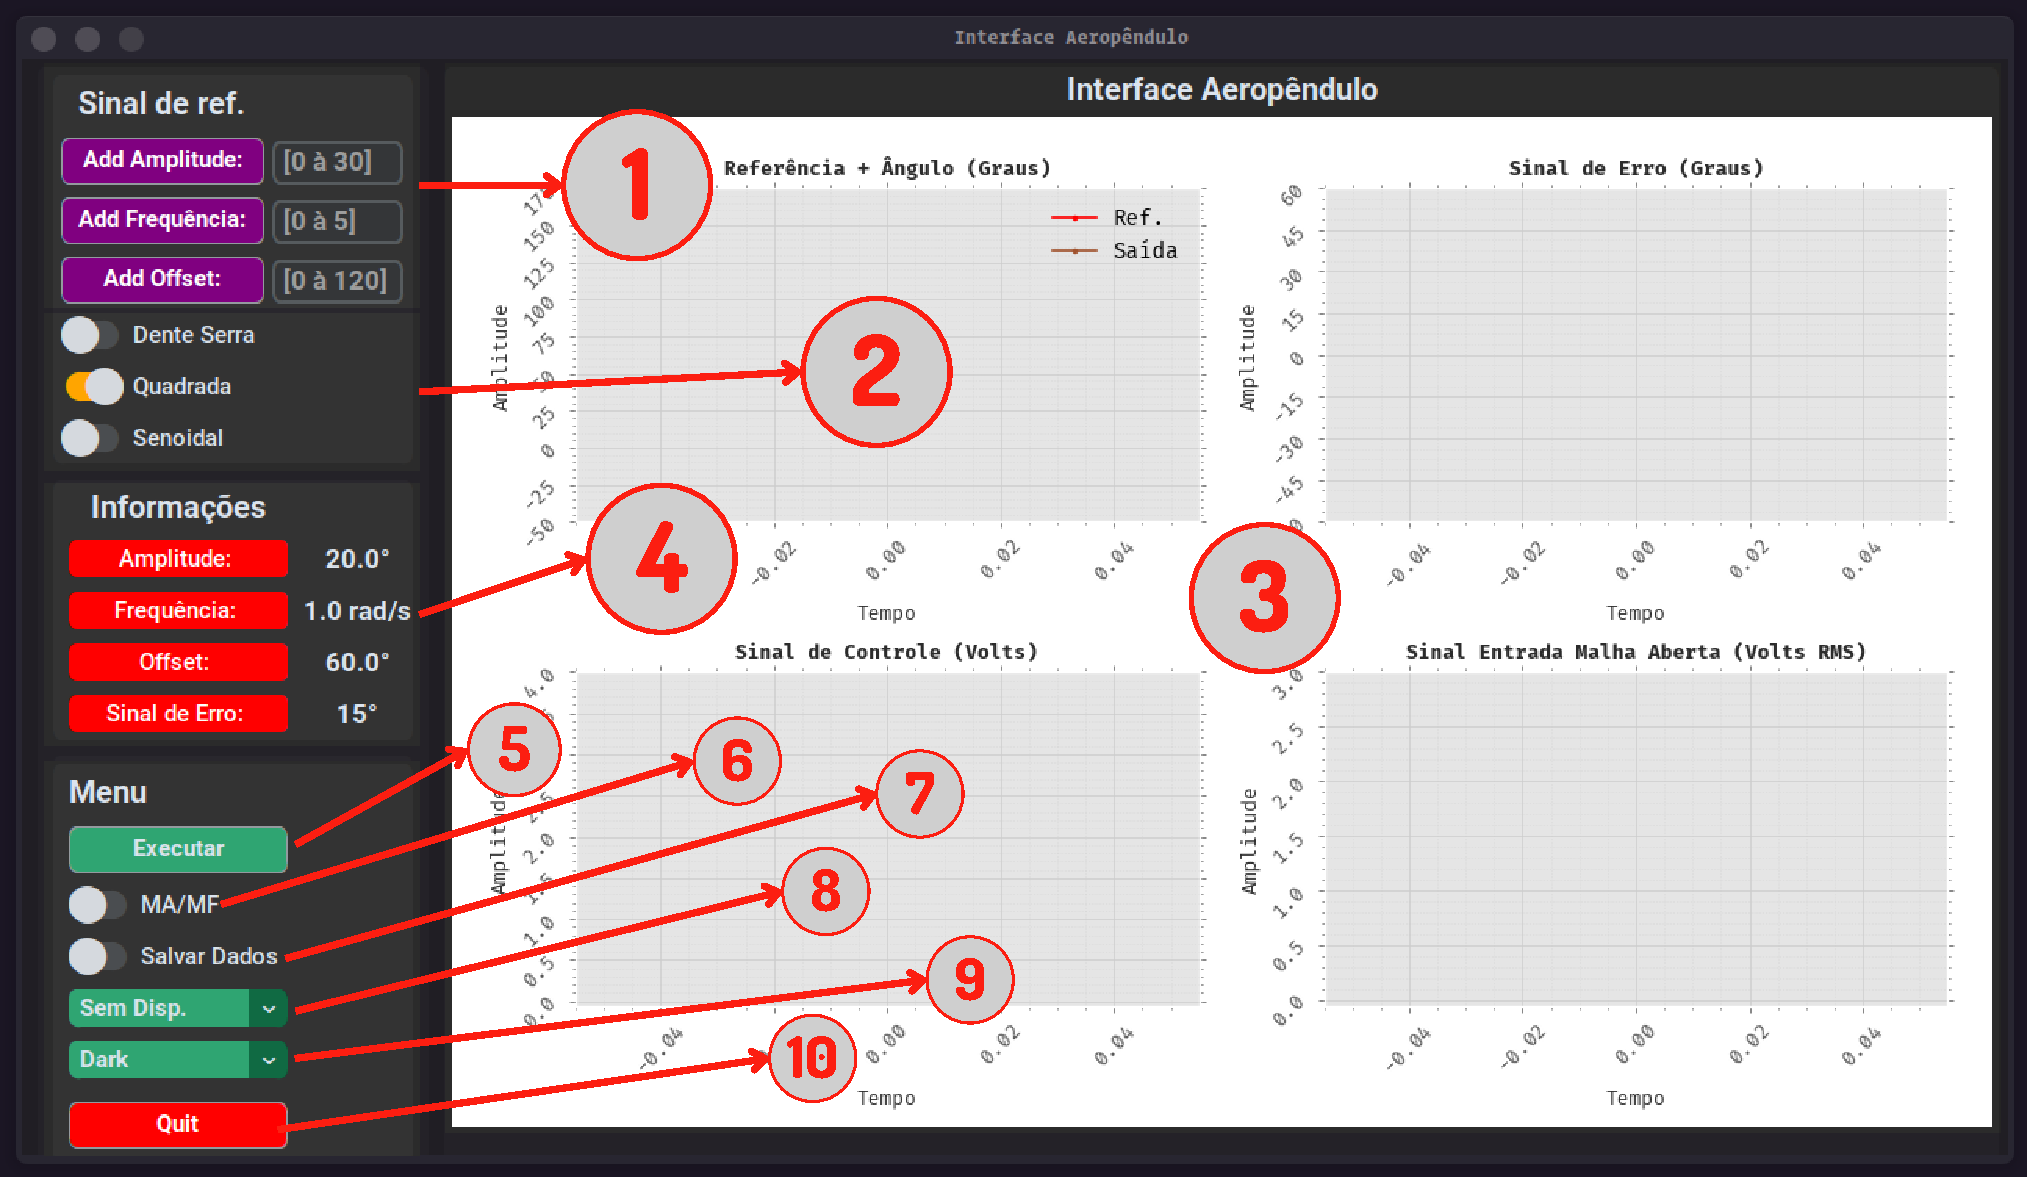
\includegraphics[width=0.95\textwidth]{Capitulos/3_hardware_softwares/3_figuras/interface_partes.pdf}}
	\caption*{Fonte: elaborado pelo autor (2023).}
	\label{fig3:image_15}
\end{figure}



\subsubsection*{\textit{Item 1: Sinal de Referência}}

Essa parte do software configura os sinais de referência aplicado ao sistema em malha fechada.


\begin{itemize}
        \setlength{\itemsep}{-2pt}
	\item  \textbf{Add Amplitude:} Configura a amplitude do sinal aplicado a entrada do sistema;
        \item  \textbf{Add Frequência:} Configura a frequência do sinal aplicado a entrada do sistema;
        \item  \textbf{Add Offset:} Configura a amplitude do offset, ponto de equilíbrio, aplicado a entrada do sistema.
\end{itemize}


\subsubsection*{\textit{Item 2: Seleção do Sinal de referência}}


\begin{itemize}
        \setlength{\itemsep}{-2pt}
	\item \textbf{Onda Serra:} Ao selecionar essa opção o sinal aplicado ao sistema será um dente de serra com as configurações de amplitude, frequência e offset conforme configurado nos três primeiros sub itens;
        \item \textbf{Quadrada:} Ao selecionar essa opção o sinal aplicado ao sistema será uma onda quadrada com as configurações de amplitude, frequência e offset conforme configurado nos três primeiros sub itens.;
        \item \textbf{Senoidal:} Ao selecionar essa opção o sinal aplicado ao sistema será uma onda senoidal com as configurações de amplitude, frequência e offset conforme configurado nos três primeiros sub itens.
\end{itemize}

\subsubsection*{\textit{Item 3: Gráficos}}

\begin{itemize}
        \setlength{\itemsep}{-2pt}
	\item \textbf{Gráficos:} Nesse item que são plotados os gráficos dos estados do sistema em tempo real.
\end{itemize}

\subsubsection*{\textit{Item 4: Informações}}

\begin{itemize}
        \setlength{\itemsep}{-2pt}
	\item \textbf{Amplitude:} Mostra a valor da amplitude do sinal de referência;
        \item \textbf{Frequência:} Mostra a valor da frequência do sinal de referência;\\
        \item \textbf{Offset:} Mostra a valor de offset aplicado ao aeropêndulo, esse valor é adicionado ao sinal de referência, dessa forma o sinal de referência varia em torno de um ponto de equilíbrio;
        \item \textbf{Sinal de Erro:} Mostra a valor do sinal de erro em tempo real.
\end{itemize}


\subsubsection*{\textit{Item 5: Menu}}

\begin{itemize}
        \setlength{\itemsep}{-2pt}
	\item \textbf{Executar:} Inicializa o ensaio, para isso é preciso que o microcontrolador esteja conectado ao computador.
\end{itemize}


\subsubsection*{\textit{Item 6: Menu}}

\begin{itemize}
        \setlength{\itemsep}{-2pt}
	\item \textbf{MA/MF:} Comuta entre o sistema em malha aberta e malha fechada.
\end{itemize}


\subsubsection*{\textit{Item 7: Menu}}

\begin{itemize}
        \setlength{\itemsep}{-2pt}
	\item \textbf{Salvar Dados:} Quando está ativado os dados são salvos em um arquivo CSV com data, hora, minuto e segundo do instante do salvamento, isso facilita que diferentes ensaios sejam realizados sem que os dados do anterior seja sobrescrito.
\end{itemize}


\subsubsection*{\textit{Item 8: Menu }}

\begin{itemize}
        \setlength{\itemsep}{-2pt}
	\item \textbf{Selecionar Dispositivo:} A aplicação detecta todos os microcontroladores conectados no computador e permite que o usuário realize a seleção do dispositivo desejado para realizar o ensaio.
\end{itemize}


\subsubsection*{\textit{Item 9: Menu}}

\begin{itemize}
        \setlength{\itemsep}{-2pt}
	\item \textbf{Selecionar Tema:} O software possui tema escuro e claro e essa opção permite que o usuário selecione entre essas duas opções.
\end{itemize}


\subsubsection*{\textit{Item 10: Menu}}

\begin{itemize}
        \setlength{\itemsep}{-2pt}
	\item \textbf{Quit:} Botão responsável por fechar a aplicação.
\end{itemize}

